\documentclass[border=10pt]{standalone}
\usepackage{tikz}
\usetikzlibrary{positioning}
\usetikzlibrary{fit}
\begin{document}
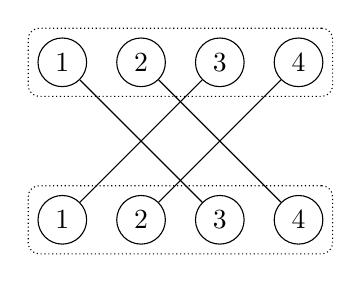
\begin{tikzpicture}]

\node (A1) at (0, 0) [draw, circle] {$1$};
\node (A2) [right of = A1, draw, circle] {$2$};
\node (A3) [right of = A2, draw, circle] {$3$};
\node (A4) [right of = A3, draw, circle] {$4$};

\node (S) [below of = A1] {};

\node (B1) [below of = S, draw, circle] {$1$};
\node (B2) [right of = B1, draw, circle] {$2$};
\node (B3) [right of = B2, draw, circle] {$3$};
\node (B4) [right of = B3, draw, circle] {$4$};


\path[-] (A1) edge (B3);
\path[-] (A2) edge (B4);
\path[-] (A3) edge (B1);
\path[-] (A4) edge (B2);

\node[draw, densely dotted, rounded corners, fit=(A1) (A4)] {};
\node[draw, densely dotted, rounded corners, fit=(B1) (B4)] {};
\end{tikzpicture}
\end{document}
